% Included inside a figure environment in Chapter 4.
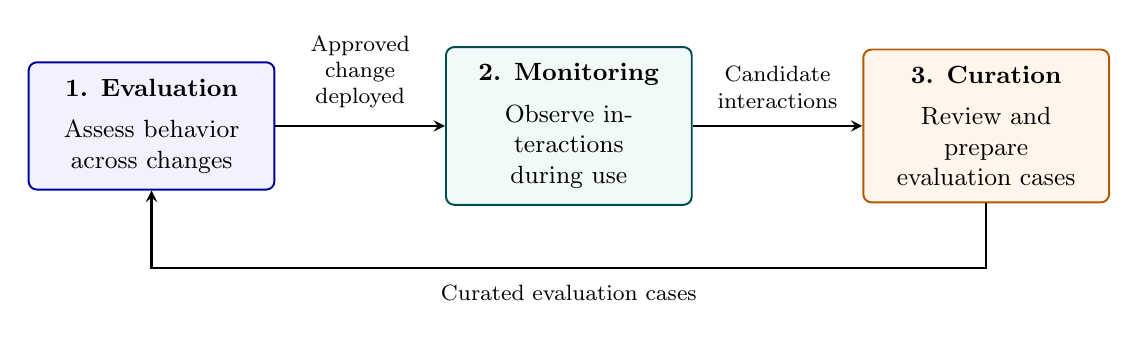
\begin{tikzpicture}[
  stage/.style={
    draw, rounded corners=3pt, line width=0.7pt,
    text width=2.7cm, minimum height=1.5cm,
    inner sep=6pt, align=center, font=\small
  },
  flow/.style={->, >=stealth, line width=0.8pt},
  transition/.style={align=center, font=\footnotesize, fill=white, inner sep=3pt}
]
  \node[stage, draw=blue!60!black, fill=blue!5] (testing) at (0,0)
    {\textbf{1. Evaluation}\\[4pt]Assess behavior\\across changes};
  \node[stage, draw=teal!60!black, fill=teal!5] (monitoring) at (5.3,0)
    {\textbf{2. Monitoring}\\[4pt]Observe interactions\\during use};
  \node[stage, draw=orange!70!black, fill=orange!8] (curation) at (10.6,0)
    {\textbf{3. Curation}\\[4pt]Review and prepare\\evaluation cases};

  \draw[flow] (testing.east) -- node[transition, above=3pt]
    {Approved\\change\\deployed} (monitoring.west);
  \draw[flow] (monitoring.east) -- node[transition, above=3pt]
    {Candidate\\interactions} (curation.west);
  \draw[flow] (curation.south) -- (10.6,-1.8)
    -- node[transition, below=3pt] {Curated evaluation cases}
    (0,-1.8) -- (testing.south);
\end{tikzpicture}
